\documentclass[../Book.tex]{subfiles}
 
\begin{document}
	\section{Perancangan Sistem}
	\subsection{\textit{Preprocessing}}
	
	\noindent Gambar \ref{fig:preprocessing} menunjukan rincian tahapan untuk proses \textit{preprocessing} yang merupakan bagian dari tahapan \textit{merging context seeds} pada Gambar \ref{fig:gambarumumsistem}.
	
	\begin{center}
		\begin{figure}[H]
			\includegraphics[width=\linewidth]{../images/preprocessing}
			\caption{Alur \textit{Preprocessing}}
			\label{fig:preprocessing}
		\end{figure}
	\end{center}

	\noindent Diketahui dokumen X(\textit{suspicious-document}) dan dokumen Y (\textit{source-document}) yang dijadikan \textit{input} untuk sistem. \textit{Preprocessing} dilakukan terhadap kedua dokumen. Sebagai contoh, proses yang ditunjukan pada Sub-Bab ini merupakan proses untuk dokumen \textit{suspicious-document00044.txt} \\

	\subsubsection{\textit{Lower casing} dan \textit{Generate Character Map}}
	\noindent \textit{Preprocessing} dimulai dengan \textit{Lower-casing}, atau mengubah seluruh alfabet yang ada pada dokumen menjadi huruf kecil. Kemudian memetakan seluruh karakter yang ada pada dokumen ke dalam \textit{char map} untuk mengetahui letak kemunculan tiap karakter pada dokumen.  \\
	
	{\fontfamily{qcr}\selectfont
		\noindent A GED is accepted by all public and most private
		colleges and universities, as well as most employers. GMAT is the most effective test available for admission to business schools.emand for qualified professionals in education and research industry is increasing. Prepare for the GRE and get going. Getting admission in a law school is now easy with the LSAT Preparation course which thoroughly teaches you the techniques and helps to build skills to take the LSAT test. The cost of the course is \$125 and is open to
		the first 40 individuals who meet the
		following
		qualifications:
		.......
	} \\

	\noindent Akan membangun \textit{char map} seperti pada Tabel \ref{example-charmap}.
	
	\begin{table}[H]
		\centering
		\caption{Contoh \textit{Char Map}}
		\label{example-charmap}
		\begin{tabular}{ll}
			\hline
			index & karakter \\ \hline
			0     & a        \\
			1     &        \\
			2     & g        \\
			3     & e        \\
			4     & d       \\
			5     &          \\
			6     & i        \\
			7     & s \\
			8	  & \\
			....  & ....\\
			12160 & \\
			12161 & g \\
			12162 & e \\
			12163 & t \\
			 \\ \bottomrule
		\end{tabular}
	\end{table}

	\subsubsection{Hapus karakter \textit{non-alphanumeric}}
	\noindent Langkah berikutnya menghapus seluruh baris yang memiliki karakter yang tidak termasuk ke dalam \textit{alphanumeric} karakter. Karakter yang termasuk ke dalam karakter \textit{non-alphanumeric} ditunjukan pada Tabel \ref{nonalphanumeric}.
	
	\begin{table}[H]
		\centering
		\caption{Daftar Karakter\textit{ Non-alphanumeric}}
		\label{nonalphanumeric}
		\begin{tabular}{|l|l|l|l|l|l|}
			\hline
			\multicolumn{1}{|c|}{`} & \multicolumn{1}{c|}{$\sim$} & !         & @              & \#           & \$   \\ \hline
			\%                      & \textasciicircum            & \&        & *              & (            & )   \\ \hline
			-                       & \_                          & +         & =              & \{           & {[} \\ \hline
			\}                      & {]}                         & |         & \textbackslash & ;            & :   \\ \hline
			"                       & '                           & \textless & ,              & \textgreater & .   \\ \hline
			?                       & /                           &           &                &              &     \\ \hline
		\end{tabular}
	\end{table}

	\subsubsection{\textit{Generate Word Map}}
	\noindent Setelah menghilangkan seluruh karakter \textit{non-alphanumeric} maka dibangun \textit{word map} dari karakter yang tersisa yang ada pada \textit{char map} dengan menyimpan informasi kemunculan awal dan akhir karakter pada kata tersebut. Tiap kata akan dibangun dengan pemisah berupa karakter spasi. Contoh dari tabel \textit{word map} ditunjukan pada Tabel \ref{wordmap}. Dengan banyak jumlah data : \textbf{129}

	\begin{table}[H]
		\centering
		\caption{Contoh \textit{Word Map}}
		\label{wordmap}
		\begin{tabular}{@{}lll@{}}
			\toprule
			Indeks awal & Indeks akhir & Kata     \\ \midrule
			0           & 0            & a    \\
			2           & 4            & ged       \\
			6           & 7           & is      \\
			9          & 16          & accepted   \\
			18          & 19           & by  \\
			...         & ...          & ... \\ \bottomrule
		\end{tabular}
	\end{table}
	
	\subsubsection{Hapus \textit{stopwords}}
	\noindent Tahap akhir \textit{preprocessing} adalah menghilangkan \textit{stopwords}. \textit{Stopwords} merupakan kata yang umum muncul, sehingga dianggap memberikan \textit{noise} pada data. Daftar \textit{stopwords} dapat dilihat pada Tabel \ref{stopwords}
	
	\begin{table}[H]
		\centering
		\caption{Daftar \textit{Stopwords}}
		\label{stopwords}
		\begin{tabular}{|l|l|l|l|l|l|l|}
			\hline
			i          & herself    & was    & because & from    & any   & t      \\ \hline
			me         & it         & were   & as      & up      & both  & can    \\ \hline
			my         & its        & be     & until   & down    & each  & will   \\ \hline
			myself     & itself     & been   & while   & in      & few   & just   \\ \hline
			we         & they       & being  & of      & out     & more  & don    \\ \hline
			our        & them       & have   & at      & on      & most  & should \\ \hline
			ours       & their      & has    & by      & off     & other & now    \\ \hline
			ourselves  & theirs     & had    & for     & over    & some  &        \\ \hline
			you        & themselves & having & with    & under   & such  &        \\ \hline
			your       & what       & do     & about   & again   & no    &        \\ \hline
			yours      & which      & does   & against & further & nor   &        \\ \hline
			yourself   & who        & did    & between & then    & not   &        \\ \hline
			yourselves & whom       & doing  & into    & once    & only  &        \\ \hline
			he         & this       & a      & through & here    & own   &        \\ \hline
			him        & that       & an     & during  & there   & same  &        \\ \hline
			his        & these      & the    & before  & when    & so    &        \\ \hline
			himself    & those      & and    & after   & where   & than  &        \\ \hline
			she        & am         & but    & above   & why     & too   &        \\ \hline
			her        & is         & if     & below   & how     & very  &        \\ \hline
			hers       & are        & or     & to      & all     & s     &        \\ \hline
		\end{tabular}
	\end{table}

	\noindent Sehingga pada akhir tahap \textit{preprocessing}, \textit{word map} yang dihasilkan ditunjukan pada Tabel \ref{cleanwordmap}. Dengan jumlah data : \textbf{84}
	
	\begin{table}[H]
		\centering
		\caption{Contoh Word Map yang Telah Dihilangkan \textit{Stopwords}}
		\label{cleanwordmap}
		\begin{tabular}{@{}lll@{}}
			\toprule
			Indeks awal & Indeks akhir & Kata     \\ \midrule
			2           & 4            & ged    \\
			9          & 16           & accepted   \\
			25			& 30		   & public \\
			41 & 47 & private \\
			49 & 56 & colleges \\
			...         & ...          & ...      \\
			12149         & 12152          & what \\ \bottomrule
		\end{tabular}
	\end{table}

	\subsection{\textit{Seed Generation}}
	\noindent Gambar \ref{fig:flowseed} menunjukan rincian tahapan untuk proses \textit{seed generation} yang merupakan bagian dari tahapan \textit{merging context seeds} pada Gambar \ref{fig:gambarumumsistem}. Seluruh proses yang ditampilkan merupakan proses yang dilakukan terhadap dokumen X \textit{(suspicious-document00017.txt)} dan dokumen Y \textit{(source-document00135.txt)}.
	
	\begin{center}
		\begin{figure}[H]
			\includegraphics[width=0.8\linewidth]{../images/seedgeneration}
			\caption{Alur \textit{Seeds Generation}}
			\label{fig:flowseed}
		\end{figure}
	\end{center}

	\subsubsection{Ekstraksi Ciri}
	Pada tahap ini dokumen X(\textit{suspicious}) dan dokumen Y(\textit{source})yang telah melalui tahap \textit{preprocessing} akan melalui proses ekstraksi ciri dengan \textit{skipword-bigram} 1-4 dengan tetap menyimpan informasi letak kemunculan karakter pada kata/\textit{token}. Dari proses ekstraksi ini akan dibangun \textit{feature map} yang ditunjukan oleh Tabel \ref{featuremap-x} seperti yang dijelaskan pada Persamaan \ref{eq:feature-extraction}. 
	
	% Please add the following required packages to your document preamble:
	% \usepackage{booktabs}
	\begin{table}[H]
		\centering
		\resizebox{\textwidth}{!}{ 
		\caption{\textit{Feature Map} Dokumen X}
		\label{featuremap-x}
		\begin{tabular}{@{}lllllll@{}}
			\toprule
			i awal & i akhir & Kata & f1                       & f2                      & f3                & f4                  \\ \midrule
			2          & 4            & ged      & *\_ged                 & *\_ged                & *\_ged          & *\_ged            \\
			9          & 16           & accepted    & ged\_accepted           & *\_accepted              & *\_accepted        & *\_accepted          \\
			25         & 30          & public        & accepted\_public                      & ged\_public                   & *\_public               & *\_public                 \\
			41         & 47          & private & all\_private & public\_private & ged\_private & *\_private  \\
			49         & 56          & colleges        & private\_colleges                      & public\_colleges                     & accepted\_colleges               & ged\_colleges \\ \bottomrule
		\end{tabular}
	}
	\end{table}
	
	\subsubsection{Seleksi Fitur/Ciri}
	Pada metode \textit{Merging Context Seeds}, fitur yang mempunyai jumlah kemunculan yang tinggi dianggap tidak relevan. Sehingga apabila ada fitur yang kemunculannya melebihi \textbf{4}, fitur akan dihapus. Nilai $4$ merupakan parameter yang sudah diuji\cite{mcs} untuk mendapatkan fitur yang optimal.\\ 
	
	\noindent Sebagai contoh : \textit{\textbf{jika} fitur \textbf{patch\_alabama} pada dokumen X muncul sebanyak \textbf{6}. Maka fitur tersebut akan dihapus seluruhnya dari feature map, baik fitur tersebut muncul di f1,f2,f3, atau f4.}
	
	
	\subsubsection{\textit{Seed Generation}}
	Pada tahap ini fitur yang ada pada dokumen X dan dokumen Y. Akan dicari irisan antara kedua dokumen tersebut dari fitur yang ada. Apabila terdapat fitur yang sama, maka akan dibangun \textit{seed set} yang merupakan titik awal pendeteksian \textit{passage} yang diplagiat pada kedua dokumen, atau disebut dengan \textit{passage reference}. Tabel \ref{seedset} menunjukan hasil \textit{seed generation} antara dokumen X \textit{(suspicious-document00017.txt)} dan dokumen Y \textit{(source-document00135.txt)}.
	
	% Please add the following required packages to your document preamble:
	% \usepackage{booktabs}
	\begin{table}[H]
		\centering
		\caption{\textit{Passage Reference} Dokumen X dan Dokumen Y}
		\label{seedset}
		\begin{tabular}{@{}lllllll@{}}
			\toprule
			$pr_{x}$ & \multicolumn{1}{c}{f} & \multicolumn{1}{c}{Kata} & \multicolumn{1}{c}{$Y_{f_{start}}$} & \multicolumn{1}{c}{$Y_{f_{end}}$} & \multicolumn{1}{c}{$X_{f_{start}}$} & \multicolumn{1}{c}{$X_{f_{start}}$} \\ \midrule
			$pr_{0}$ & gmat\_test       		& test                   	& 1181                    	& 1199                    	& 130                   & 133	\\
			$pr_{1}$ & gmat\_questions       	& questions             	& 1191	                    & 1199                    	& 1043                  & 1051	\\
			$pr_{2}$ & gmat\_questions       	& questions                 & 1191  	               	& 1199                    	& 1103                  & 1111	\\
			$pr_{3}$ & gmat\_questions		 	& questions					& 1191						& 1199						& 1308					& 1316 	\\
 			...		 & ...                   	& ...                      	& ...                   	& ...                   	& ...                   & ...	\\
			$pr_{461}$ 	& takers\_right         & right                   	& 1300                   	& 1304                   	& 9868                 & 9872          \\ \bottomrule         
		\end{tabular}
	\end{table}
	
	Kolom $Y_{f_{start}}$ menunjukan kemunculan awal kata pada \textit{feature map} pada dokumen Y, sedangkan $Y_{f_{end}}$ menunjukan akhir kemunculan kata pada \textit{feature map} pada dokumen Y. Sedangkan $X_{f_{start}}$ dan $X_{f_{end}}$ menunjukan kemunculan pada dokumen X. Seluruh letak kemunculan pada Tabel \ref{seedset} didapatkan dari proses ekstraksi ciri.
	
	\subsection{Merging}
	
	\noindent Gambar \ref{fig:merge} menunjukan rincian tahapan untuk proses \textit{merging} yang merupakan bagian dari tahapan \textit{merging context seeds} pada Gambar \ref{fig:gambarumumsistem}.
	
	\begin{center}
		\begin{figure}[H]
			\includegraphics[scale=0.4]{../images/merge}
			\caption{Alur \textit{Merging}}
			\label{fig:merge}
		\end{figure}
	\end{center}

	\noindent Proses \textit{merging} merupakan proses dimana sistem akan meng-\textit{cluster} setiap \textit{passage reference} menggunakan algoritma \textit{single linkage clustering}. Kriteria \textit{merge} yang digunakan adalah jarak terpendek antara 2 \textit{passage reference} dari kumpulan \textit{passage reference} yang ada. Proses \textit{merging} akan terhenti apabila memenuhi salah satu dari dua kondisi terminasi berikut : 
	
	\begin{enumerate}
		\item Jarak terpendek  $\leq \tau; \tau = 7$.\\
		Nilai 7 dianggap nilai yang paling optimal dari pengujian sementara dengan range nilai 5 - 15.
		\item Jumlah cluster $=1$. \\
		Yang berarti  seluruh \textit{seed} yang didapat sudah masuk kedalam satu \textit{cluster}.
		\item Jumlah cluster $=0$. \\
		Tidak terdapat \textit{seed} pada proses \textit{seed generation} sebelumnya.
		
	\end{enumerate} 
	
	\noindent Tabel \ref{prxpr} menunjukan jarak antar \textit{seed} atau \textit{passage reference} yang didapat dari proses \textit{seed generation}.
	
	\begin{table}[H]
		\centering
		\caption{Jarak Antar \textit{Passage Reference}}
		\label{prxpr}
		\begin{tabular}{l|llllllll}
			Dist      & $pr_{0}$              & $pr_{1}$              & $pr_{2}$              & $pr_{3}$              & $pr_{4}$              & ...                     & $pr_{15}$               & ...                     \\ \hline
			$pr_{0}$  & \multicolumn{1}{c}{x} & 41.6                  & 44.2                  & 53.3                  & 178.2                 & ...                     & ...                     & ...                     \\
			$pr_{1}$  & 41.6                  & \multicolumn{1}{c}{x} & 1.8                   & 8.1                   & 90.2                  & ...                     & ...                     & ...                     \\
			$pr_{2}$  & 44.2                  & 1.8                   & \multicolumn{1}{c}{x} & 6.3                   & 88.3                  & ...                     & ...                     & ...                     \\
			$pr_{3}$  & 53.3                  & 8.1                   & 6.3                   & \multicolumn{1}{c}{x} & 81.6                  & ...                     & ...                     & ...                     \\
			$pr_{4}$  & 178.2                 & 90.2                  & 88.3                  & 81.6                  & \multicolumn{1}{c}{x} & ...                     & ...                     & ...                     \\
			...       & ...                   & ...                   & ...                   & ...                   & ...                   & \multicolumn{1}{c}{...} & ...                     & ...                     \\
			$pr_{13}$ & ...                   & ...                   & ...                   & ...                   & ...                   & ...                     & {\color[HTML]{FE0000} 0.0} & ...                     \\
			...       & ...                   & ...                   & ...                   & ...                   & ...                   & ...                     & ...                     & \multicolumn{1}{c}{...}
		\end{tabular}
	\end{table}

	\noindent Dari hasil \textit{loop} pertama diketahui jarak antara \textit{passage reference} terdekat ada di $pr_{13} \text{ dan } pr_{15}$ dengan jarak $0.0$, maka $pr_{13} \text{ dan } pr_{15}$ akan di \textit{merge}. Data kandidat yang ditunjukan pada Tabel \ref{kandidat-merge}. Nilai kemunculan pada dokumen X dan dokumen Y didapatkan dari proses ekstraksi ciri pada tahap sebelumnya.
	
	% Please add the following required packages to your document preamble:
	% \usepackage{booktabs}
	\begin{table}[H]
		\centering
		\caption{Kandidat \textit{Passage Reference} yang Akan Di-\textit{merge}}
		\label{kandidat-merge}
		\begin{tabular}{@{}llllll@{}}
			\toprule
			$pr_{x}$  & Kata   & $Y_{f_{start}}$ & $Y_{f_{end}}$ & $X_{f_{start}}$ & $X_{f_{end}}$ \\ \midrule
			$pr_{13}$ & reasoning & 1861     & 1869   & 3874     & 3882  \\
			$pr_{15}$ & reasoning & 1861     & 1869   & 3874     & 3882   \\ \bottomrule
		\end{tabular}
	\end{table}

	\noindent Pada Tabel \ref{hasil-merge} terlihat bahwa nilai $X_{f_{start}}$ dan $X_{f_{end}}$ diambil dari titik terendah untuk $X_{f_{start}}$, dan titik terjauh untuk $X_{f_{start}}$ dikarenakan penggabungan dua buah \textit{passage reference}. Dikarenakan \textit{passage reference} yang akan digabung merupakan fitur yang ada pada kata yang sama, sehingga tidak ada perubahan untuk nilai kemunculannya
	
	\begin{table}[H]
		\centering
		\caption{Hasil Merge}
		\label{hasil-merge}
		\begin{tabular}{@{}llllll@{}}
			\toprule
			$pr_{x}$  & Kata   & $Y_{f_{start}}$ & $Y_{f_{end}}$ & $X_{f_{start}}$ & $X_{f_{end}}$ \\ \midrule
			$pr_{13,15}$ & reasoning, reasoning & 1861     & 1869   & 3874     & 3882   \\ \bottomrule
		\end{tabular}
	\end{table}

	\noindent Proses akan diulang hingga tidak ada jarak antar \textit{passsage reference} yang melebihi $\tau$. Tabel \ref{prxpr} menunjukan jarak terpendek antar \textit{passage reference} pada \textit{looping} pertama. 

	\subsection{\textit{Filtering}}
	
	Pada tahap ini \textit{cluster} akhir akan dipilihi, apabila \textit{cluster} mempunyai jumlah anggota atau \textit{passage reference} $\geq \tau; \tau = 15$\cite{mcs} maka $pr_{n..m}$ dianggap menjadi bagian yang diplagiat ($r$).
	
	\subsection{\textit{Output}}
	
	Dari tahap \textit{filtering} didapat lokasi tindak plagiat, pada tahap \textit{output} ini mengembalikan bagian dari kedua dokumen. \\
	
		% \usepackage{booktabs}
	\begin{table}[H]
		\centering
		\caption{$r \in R$}
		\label{output}
		\begin{tabular}{@{}lllll@{}}
			\toprule
			r & $Y_{f_{start}}$ & $Y_{f_{end}}$ & $X_{f_{start}}$ & $X_{f_{end}}$ \\ \midrule
			$r_{1}$ & 8       & 979   & 3805    & 4427  \\
			$r_{2}$ & 1160    & 1620  & 9073    & 9461  \\
			$r_{3}$ & 1719    & 2134  & 8269    & 8580  \\ \bottomrule
		\end{tabular}
	\end{table}
	
	\noindent Tabel \ref{output} menunjukan $r \in R$ pada \textit{pair suspicious-document00044.txt-source-document01326.txt} yang didapat dari hasil akhir \textit{merging} yang didapat dari tahap sebelumnya. Kemudian dibangkitkan nilai kemunculannya mejadi teks pada dokumen sesungguhnya, sehingga hasil yang dimunculkan ditunjukan seperti pada Tabel \ref{output-real}.
	
		\newpage
	
	% Please add the following required packages to your document preamble:
	% \usepackage{booktabs}

		\begin{longtable}{@{}lp{7cm}p{7cm}@{}}
			\caption[\textit{Output} akhir berupa teks yang diplagiat]{\textit{Output} akhir berupa teks yang diplagiat} \label{output-real} \\
			\hline
			$r$       & Teks Pada Dokumen X                                                                                                                                                                                                                                                                                                                                                                                                                                                                                                                                                                                                                           & Teks Pada Dokumen Y                                                                                                                                                                                                                                                                                                                                                                                                                                                                                                                                                                                                                                                                                                                                                                                                                                                                                                                                                                                       \\ \hline
			$r_{1}$ & questions of three question types -- reading comprehension, critical reasoning, and sentence correction. you are allowed 75 minutes to complete this entire section. verbal section each passage engages with a specialized topic or opinion in either the humanities, social sciences, science, or business, but no specific outside knowledge of the material is required; all questions refer to what is stated or implied in the text. the directions for these questions look like this: each passage is followed by questions about its content. after reading a passage, select the best answer to each question among the five choice & comprehension   this is a partial free sample of our prep guide. to view the remainder of this page, purchase the .   typically, your verbal test will include 4 reading comprehension passages, with 3 to 4 questions per passage, for a total of 12 to 14 questions of the 41 verbal questions. each passage engages with a specialized topic or opinion in either the humanities, social sciences, science, or business, but no specific outside knowledge of the material is required; all questions refer to what is stated or implied in the text. the directions for these questions look like this: each passage is followed by questions about its content. after reading a passage, select the best answer to each question among the five choices. answer all questions following a passage on the basis of what the passage states or implies.directions: a passage and a corresponding question look like this: the screen will split into two with the passage on the left and the question \\
			$r_{2}$ & computer-adaptive test) so the questions will begin at an intermediate skill level and . in general, average test takers will get about 50\% right of the questions right. as result, higher scorers are effectively taking a completely different test from lower scorers and their strategies will be adjusted accordingly. higher scorers will get longer and more challenging essays and question                                                                                                                                                                                                                                         & computer-adaptive test) so the questions will begin at an intermediate skill level and . in general, average test takers will get about 50\% right of the questions right. as result, higher scorers are effectively taking a completely different test from lower scorers and their strategies will be adjusted accordingly. higher scorers will get longer and more challenging essays and questions. this chapter has sections specifically designed to help higher scorer                                                                                                                                                                                                                                                                                                                                                                                                                                                                                                                             \\
			$r_{3}$ & adapt to your performance by changing in difficulty   if you are extremely good at sentence correction and weak at reading comp and critical reasoning.... guess what? your skill in sentence correction will make the gmat deliver you very hard reading comp and critical reasoning questions. the moral of the stor                                                                                                                                                                                                                                                                                                                        & adapt to your performance by changing in difficulty   if you are extremely good at sentence correction and weak at reading comp and critical reasoning.... guess what? your skill in sentence correction will make the gmat deliver you very hard reading comp and critical reasoning questions. the moral of the story.... be balanced on verbal and skilled at all three question types.how the cat impacts verbal difficult                                                                                                                                                                                                                                                                                                                                                                                                                                                                                                                                                                            \\ \hline
		\end{longtable}

	\subsection{Evaluasi}
	Evaluasi dilakukan untuk mengukur perfomansi sistem yang dibangun. Evaluasi pada tahap ini dilakukan pada level \textit{pair}. Cara untuk mengukur perfomansi adalah dengan membandingkan $r \in R$ keluaran sistem, dengan $s \in S$ dari \textit{dataset}. Tiap elemen $R$ akan dicari irisan untuk tiap elemen $S$ untuk mendapatkan nilai \textit{\textbf{True Positive}}. Sedangkan elemen $R$ dianggap \textit{\textbf{Test Outcome Positive}} dan elemen $S$ sebagai \textit{\textbf{Condition Positive}}. Gambar \ref{fig:perfomansi} menunjukan bagaimana perhitungan untuk nilai \textit{\textbf{True Positive, Test Outcome Positive, Condition Positive}}. Dimana pada Gambar \ref{fig:perfomansi} menunjukan area plagiat yang ada pada \textit{dataset} dan area plagiat yang dideteksi oleh sistem.
	
	\begin{center}
		\begin{figure}[H]
			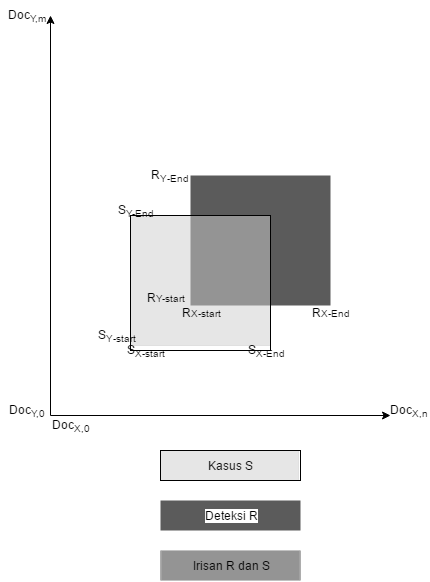
\includegraphics[width=\linewidth]{../images/perfomansi}
			\caption{Perhitungan Nilai Perfomansi}
			\label{fig:perfomansi}
		\end{figure}
	\end{center}

	\noindent Tabel \ref{s} merupakan \textit{set case} $s \in S$ atau bagian yang dinyatakan plagiat untuk \textit{pair suspicious-document00044.txt-source-document01326.txt} yang diapat dari \textit{dataset}.
	
	\begin{table}[H]
		\centering
		\caption{$s \in S$}
		\label{s}
		\begin{tabular}{lllll}
			\hline
			s       & $Y_{f_{start}}$ & $Y_{f_{end}}$ & $X_{f_{start}}$ & $X_{f_{end}}$ \\ \hline
			$s_{1}$ & 298             & 741           & 3975            & 4418          \\
			$s_{2}$ & 1143            & 1548          & 9028            & 9433          \\
			$s_{3}$ & 1713            & 2032          & 8240            & 8559          \\ \hline
		\end{tabular}
	\end{table}
	
	\noindent Sedangkan Tabel \ref{rcaps} menunjukan jumlah luas irisan area plagiat atau \textit{passage} dari $r \in R$ dan $s \in S$.
	
	\begin{table}[H]
		\centering
		\resizebox{\textwidth/2}{!}{ 
		\caption{$R \cap S$}
		\label{rcaps}
		\begin{tabular}{l|lll}
			$\pi(r_{x} \cap s_{y})$ & $r_{1}$   & $r_{2}$   & $r_{3}$   \\ \hline
			$s_{1}$ & 1772 & 0     & 0     \\ 
			$s_{2}$ & 0     & 1496 & 0     \\ 
			$s_{3}$ & 0     & 0     & 1204 
		\end{tabular}
		}
	\end{table}

	\noindent Sehingga perhitungan perfomansi untuk \textit{pair suspicious-document00044.txt-source-document01326.txt} ditunjukan pada Tabel \ref{res-perfomansi}.
	
	\begin{table}[H]
		\centering
		\caption{Contoh Perhitungan Perfomansi pada Level 1 Dokumen}
		\label{res-perfomansi}
		\begin{tabular}{|l|l||l|}
			& True Positive                      & 4474 \\
			Condition Positive    & True Positive + False Negative     & 4468    \\
			Test Outcome Positive & True Positive + False Positive     & 6334    \\
			Precision             & True Positive / Prediction Positive & 0.706   \\
			Recall                & True Positive / Condition Positive & 0.958   \\
			$F_{1}$                    & $2 \cdot \cfrac{prec(S,R) \cdot rec(S,R)}{prec(S,R) + rec(S,R)}$                                   & 0.813  
		\end{tabular}
	\end{table}
	
	\noindent Dari Tabel \ref{res-perfomansi} didapat informasi bahwa \textit{test accuracy} atau nilai $F_{1}$ untuk \textit{pair suspicious-document00044.txt-source-document01326.txt} adalah 0.813.

\end{document}